\section{Metody detekce a současná řešení pro detekci chodců}
V této kapitole budou popsány přístupové techniky a současný stav techniky detekce chodců nejpoužívanějších a nejznámějších detekčních metodik. Všechny tyto metodiky jsou dostupné minimálně v jedné knihovně, použité v této práci.  

\subsection{Metody detekce}
Navzdory všem výzvám a problémům detekci chodců, zůstává tato oblast výzkumu stále aktivní a byla navržena řada přístupových technik.

\subsubsection{Holistická detekce}

Tyto detektory jsou určeny pro vyhledávání chodců skenováním celého snímku. Detektor by označil obrázek za kladný, jestliže vlastnosti uvnitř lokálního okna splňují určitá kritéria. Některé techniky využívají globálních funkcí (hranové šablony\cite{edgeTemplate}), některé lokálních funkcí (histogram orientovaných gradientů\cite{hog:dalal}). Nevýhodou tohoto přístupu je, že výkon může být snadno ovlivněný komplexním nebo chaotickým pozadím a okluze.

\subsubsection{Detekce založena na částech}

Chodci jsou modelování jako kolekce částí. Část hypotézy jsou prvně generovány učením lokálních vlastností, které zahrnují okraje\cite{edgelet} a orientační vlastnosti \cite{orientationFeatures}. Tyto části jsou následně spojeny tak, aby vytvořily co nejlepších sestavu již stávajících hypotéz pro chodce. I když je tato přístupová metoda atraktivní, samotná detekce je obtížná. Implementace této metody vychází ze standardního postupu zpracování obrazových dat, kdy nejprve vytvoříme hustě vzorkovanou obrazovou pyramidu, vypočteme její vlastnosti v každém měřítku provedeme klasifikaci na všech možných místech, a nakonec provedeme non-maxima supression pro vytvoření konečné sady ohraničujících boxů.\cite{partModels} 

\subsubsection{Detekce založena na výstřižku}

Detektor se během trénování naučí dokument místního vzhledu kódu. V detekční procesu, extrahované lokální vlastnosti se porovnávají s položkami tohoto dokumentu a každá shoda vyjadřuje jeden hlas pro hypotézu chodce. Konečný výsledky detekce lze získat dalším vylepšením těchto hypotéz. Výhodou této přístupové techniky je, že vyžaduje pouze malý počet tréninkových vzorků. Klasifikaci využívající tuto metodu přístupu v kombinaci detekce a segmentace navrhnul Leibe a kolektiv\cite{leibe}.

\subsubsection{Detekce založena na pohybu}

Tuto přístupovou metodu můžeme použít, pokud jsou pro to vhodné podmínky (statická kamera, stacionární světelné podmínky apod.) a to odčítáním pozadí.  Tato procedura zdůrazňuje siluety každého pohybujícího se prvku ve scéně, včetně lidí. Za účelem analyzovat tyto siluety, zda-li se jedná o člověka, byl vyvinut algoritmus na univerzitě v Lutychu\cite{motionAlg1}\cite{motionAlg2}.

\subsubsection{Detekce pomocí více kamer}

Integraci více kalibrovaných kamer pro detekci více chodců navrhnul Fleuret a kolektiv\cite{multiCameras}. Detektor vytváří mapu pravděpodobnostního obsazení (POM), které poskytuje odhad pravděpodobnosti každé buňce, která bude obsazena osobou. Při dvou až čtyř synchronizovaných video streamů pořízených v úrovní očí a z různých úhlů, může tato metoda efektivně kombinovat generativní model s dynamickým programováním k přesnému sledování až šesti osob přes 1000 snímků i přes významné okluze nebo změnám osvětlení. Touto metodou také dokážeme získat metricky přesnou trajektorii pro každého z nich.

\subsection{Současná řešení pro detekci chodců}
Od samého počátku tohoto vědeckého odvětví rozpoznávání v obrazech uplynulo již mnoho let. Během těchto let bylo vynalezeno mnoho přístupových technik a metod pro úspěšně detekování chodců v obrazech. V následujících podkapitolách budou popsány některé z nich, které mají největší úspěch v pravděpodobnosti v detekci.

\subsubsection{Mixtura Gaussiánů}

Mixtura Gaussiánů (\textit{MOG - Gaussian mixture model background subtraction}) \cite{mog:zivkovic} je metoda substrakce pozadí.  Je běžná a~široce používaná technika pro generování masky v~popředí pomocí statických kamer. Jak už jde poznat z~názvu, algoritmus vypočítá masku v~popředí a~odečítá ji mezi aktuálním rámcem (obrázek \ref{mog_scheme}) a~modelem pozadí obsahující statickou část scény nebo obecně vše, co se dá považovat za statické pozadí vzhledem k~charakteristice pozorované scény. 

Skládá se ze dvou hlavních kroků:
 \begin{enumerate}
    \item{Inicializace pozadí;}
    \item{Aktualizace pozadí.}
 \end{enumerate}
 V~prvním kroku je vypočítán model pozadí, zatímco v~druhém kroku je tento model aktualizován, aby se přizpůsobil možným změnám ve scéně. \cite{openCV:MOG}
Jeho chování a citlivost detekce lze ovlivnit nastavením parametrů a jeho novější verze v knihovně OpenCV disponuje i parametrem pro detekci stínů v obraze.
\begin{figure}[H]
  \centering
  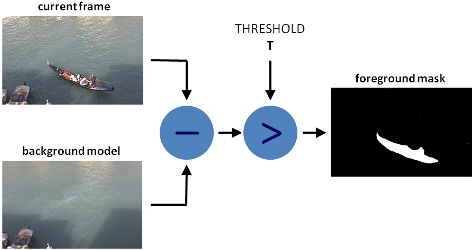
\includegraphics[width=12cm]{figures/mog_scheme}
  \caption{Schéma metody substrakce pozadí \cite{openCV:MOG}}
  \label{mog_scheme}
\end{figure}


\subsubsection{Konvexní obal}

Konvexní obal (\textit{Convex hull}), je metoda sloužící k~obalování pixelů v~prahovém obraze. Funkce používá Sklanskýho algoritmus \cite{openCV:sklansky} a~má složitost  $O(N \log(N))$.  Vstupem je množina bodů uložená v~matici nebo vektoru a~výstupem je vektor indexů nebo vektor bodů. Tyto body, které vytvářejí právě zmiňovaný konvexní obal se nakreslí do obrazu. \\
Příklad konvexního obalu je na obrázku \ref{fig:convexHull}.
\begin{figure}[H]
\centering
\begin{minipage}{.5\textwidth}
  \centering
  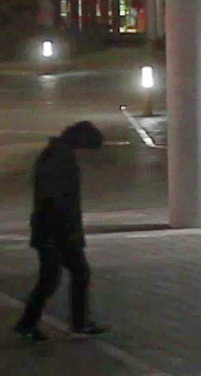
\includegraphics[width=.5\linewidth]{figures/Hull_Original}
  \caption*{Před aplikací}
  \label{fig:original}
\end{minipage}%
\begin{minipage}{.5\textwidth}
  \centering
  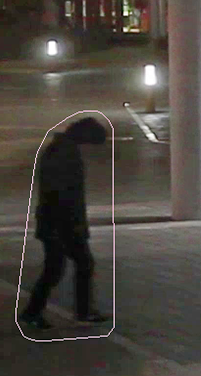
\includegraphics[width=.5\linewidth]{figures/Hull_Result}
  \caption*{Po aplikaci}
  \label{fig:result}
\end{minipage}
\caption{Aplikace konvexního obalu v~obraze}
\label{fig:convexHull}
\end{figure}

\subsubsection{Histogram orientovaných gradientů}

Tato metoda vznikla v roce 2005 za účelem detekování chodců v obrazech a je založena na histogramech orientovaných gradientů (\textit{HOG - Histogram of Oriented Gradients}). Autoři této metodiky jsou N. Dalal a B. Triggs \cite{hog:dalal}. Základní myšlenkou je, že místní vzhled a~tvar objektu může být často charakterizován distribucí intenzity gradientů nebo směry hran, aniž by byly přesně známy odpovídající gradientové nebo hranové polohy.  
Prvním krokem před samotným výpočtem příznaků by mělo dojít k zajištění normalizaci barev a gamy, v případě černobílých obrázků normalizaci kontrastu. Tento krok může být ovšem vynechán, jak zdůrazňují autoři Dalal a Triggs. Normalizace deskriptorů dosahují stejného výsledku, a tedy předběžné zpracování obrázku má malý vliv na výkon. Místo toho je prvním krokem výpočet gradientních hodnot. Nejběžnější metodou je aplikování 1-D derivační masky v jednom nebo obou horizontálních a vertikálních směrů. Autoři také experimentovali s komplexnějšími masky, jako je například $3x3$ Sobelova maska nebo diagonální masky, avšak tyto masky se prokázaly jako méně účinné. Stejně tak neúčinné bylo použití jakéhokoliv vyhlazení obrazu před aplikací derivační masky. Tedy nejlepší kombinací parametrů bylo použití konvolucí Gaussovského filtrování $\sigma = 0$ na obraze $I$ s maskou $[-1, 0, 1]$, $[-1,0,1]^\top$:
\begin{equation}
\centering
 \label{eq:hogMask}
 \begin{aligned}
I_x = I * [-1, 0, 1], \\
I_y = I * [-1, 0, 1]^\top
 \end{aligned}
\end{equation}
kde:
\begin{itemize}[label=]
  \item $*$: konvoluce,
  \item $I$: obraz.
\end{itemize}

Druhém kroku dochází k vytvoření histogramu v každé buňce. Každý pixel v buňce má svou váhu, který se podílí na vytvoření orientovaného histogramu, založeného na hodnotách nalezených ve výpočtu gradientu. Samotné buňky jsou rovnoměrně rozloženy do 9 kanálů (binů) po \ang{20}. Pokud buňka vyjde na pomezí úhlu, přičte se její magnituda do obou těchto binů.
Tyto buňky spojíme do větších propojených bloků z důvodu normalizace osvětlení a kontrastu. Pro chodce se používá L2-norm normalizace \ref{eq:normHog}. Tyto bloky se typicky překrývají, což znamená, že každá buňka přispívá více než jednou do finálního deskriptoru. Proces zpracování deskriptoru je ilustrován na obrázku \ref{hog_chain}. Existují dvě varianty spojení bloků, tzv. obdélníkové bloky (R-HOG) a kruhové bloky (C-HOG), viz obrázek \ref{variants_block}.  
\begin{equation}
\centering
 \label{eq:normHog}
 \begin{aligned}
L2-norm&: \qquad  f =& \frac{v}{\sqrt{\lVert v \lVert_2^2 + e^2}} \\
L1-sqrt&: \qquad  f =& \sqrt{\frac{v}{\lVert v \lVert_1 + e}}
 \end{aligned}
\end{equation}
Nechť $v$ je nenormalizovaný vektor obsahující všechny histogramy v daném bloku, $\lVert v \lVert_k$ je jeho k-norm pro $k = 1,2$, a $e$ je malá konstanta.
 \begin{figure}[H]
\centering
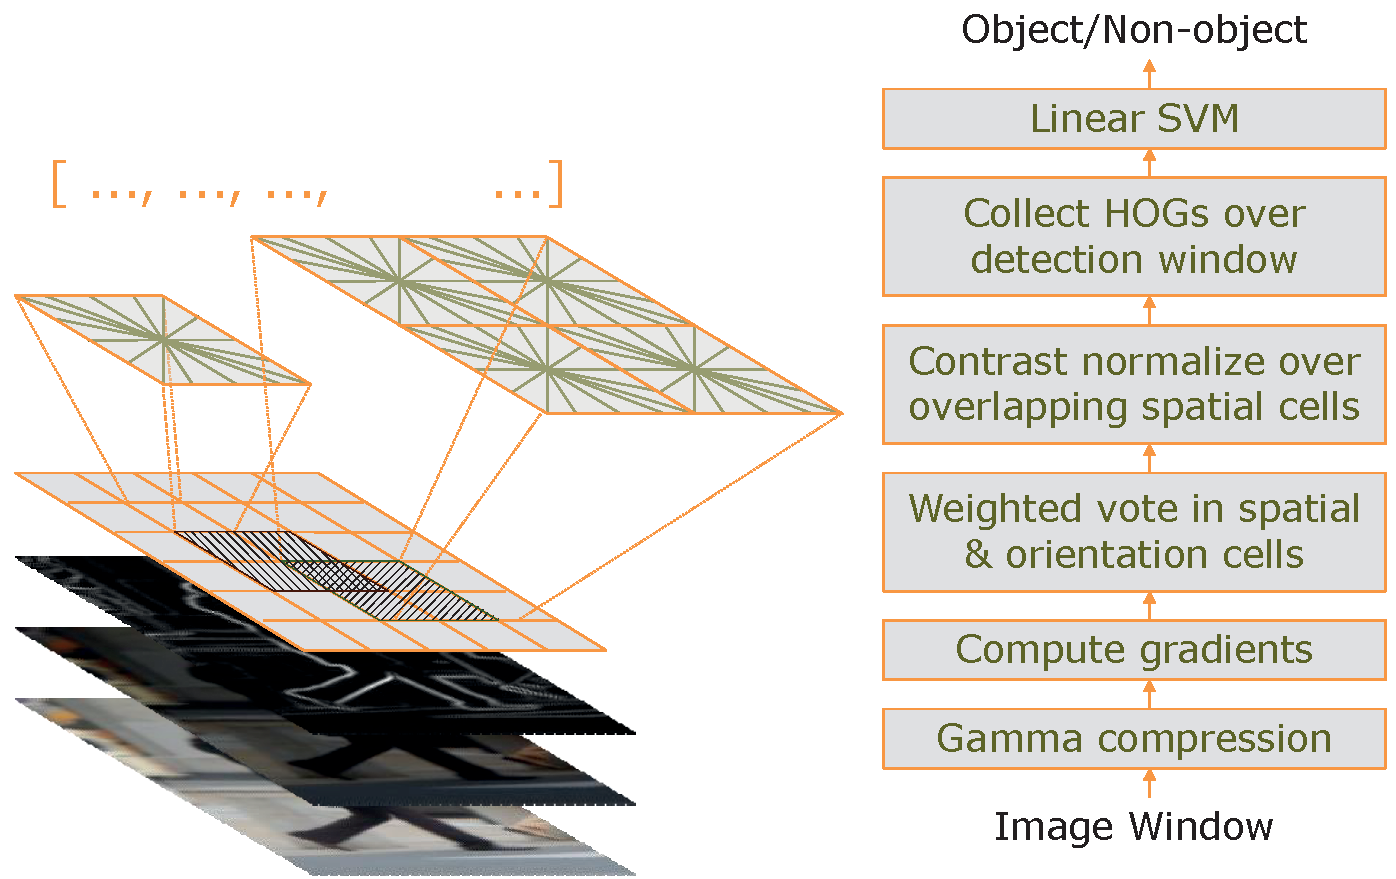
\includegraphics[width=15cm]{figures/hog_pipeline}
\caption{Procesní řetezec výpočtu deskriptoru \cite{hog:dalal}}
\label{hog_chain}
\end{figure}

\textbf{C-HOG} (Kruhové HOG bloky) - lze nalézt ve dvou variantách: \textit{s jedinou, centrální buňkou} a \textit{úhlově rozdělenou centrální buňkou}. Dají se popsat čtyřmi parametry: počtem úhlů a radiálních kanalů (binů), poloměrem centrálního binu a faktorem roztažení pro poloměr dalších radiálních binů.  Tyto bloky se podobají deskriptorům kontextu tvarů (shape context descriptors \cite{shapeContext}), ale C-HOG obsahují buňky s několika orientovanými kanály, zatím co shape context využívají přítomnost jediné hrany.

\textbf{R-HOG} (Obdélníkové HOG bloky) - tyto bloky jsou v praxi nejčastěji používané a reprezentují se třemi parametry: \textit{počet buněk na blok}, \textit{počet pixelů na buňku} a \textit{počet binů (kanálů) na jeden histogram}. Bloky se zdají trochu podobné deskriptorům transformací příznaků invariantní vůči měřítku (scale-invariant feature transform SIFT \cite{siftPaper}). Avšak liší se výpočtem bloků. R-HOG bloky jsou vypočteny v hustých mřížkách v libovolném měřítku bez zarovnání orientace, zatímco SIFT deskriptory obvykle v řídkých, obrazové body invariantní vůči měřítku jsou otočeny, aby přiléhaly orientaci. R-HOG bloky se také používají pro kódování informací. 
\begin{figure}[H]
  \centering
  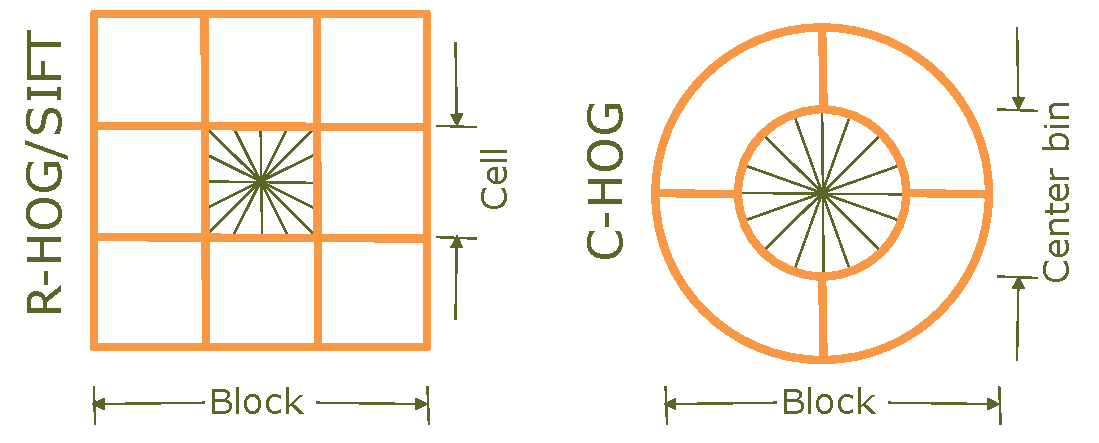
\includegraphics[width=12cm]{figures/hog_variants.pdf}
  \caption{Varianty geometrie spojení bloků \cite{hog:dalal}}
  \label{variants_block}
\end{figure}
V knihovně OpenCV existuje funkce ``detectMultiScale'', která pomocí \textbf{posuvného okénka} (sliding window) projde napříč celým obrazem a v každém tomto okně se vypočítávají vlastnosti. Jeho velikost můžeme definovat pomocí parametru, standardní velikost je $64x120$ a následující popis a výpočty budou odpovídat této velikosti posuvného okna.  

V tomto okně se obrázek rozdělí na $8x8$ bloků a v každém bloku se vypočte histogram a jeho hrany rozdělíme do 9 binů. Vyjde nám vektor o velikosti 9 a tyto vektory spojíme do bloků o velikosti $16x16$ a normalizujeme je na velikost 1, aby byly nezávislé na osvětlení, dostaneme tedy vektor o velikosti 36. Na konci tohoto procesu všechny vektory spojíme a získáme vektor všech příznaků z konkrétního vzorku nebo z oblasti zájmu posuvného okénka. Obrázek \ref{fig:hogCalc} zobrazuje vstup vzorku pro vypočítání jeho příznaků neboli orientovaných hran, kde nejprve obrázek převedeme do černobílé barvy, provedeme normalizaci kontrastu a gamy a následně vypočítáme jeho vektor příznaků.

Tato metodika se běžně používá s lineárním SVM klasifikátorem, a tak je velmi účinná pro jakoukoliv detekci. 
Ukázka dělení obrazového okna je na obrázku \ref{hog_cells}.

 \begin{figure}[H]
\centering
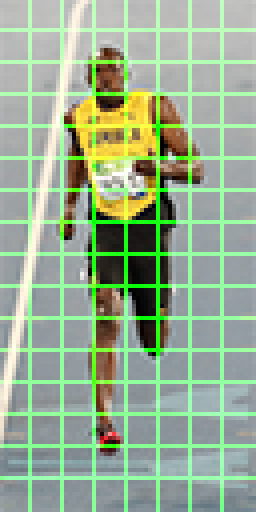
\includegraphics[width=3.6cm]{figures/hog_cells}
\caption{Rozdělení obrazu do $8\times8$ buněk. \cite{hog:obr}}
\label{hog_cells}
\end{figure}

\begin{figure}[H]
\centering
\begin{minipage}{.3\textwidth}
  \centering
  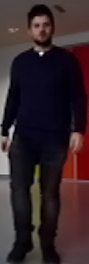
\includegraphics[width=.5\linewidth]{figures/hog_input}
  \caption*{Vstupní obrázek}
  \label{fig:hog_input}
\end{minipage}%
\begin{minipage}{.3\textwidth}
  \centering
  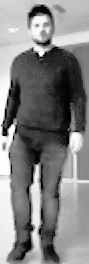
\includegraphics[width=.5\linewidth]{figures/hog_histogram_before}
  \caption*{Normalizace kontrastu}
  \label{fig:hog_contrast}
\end{minipage}%
\begin{minipage}{.3\textwidth}
  \centering
  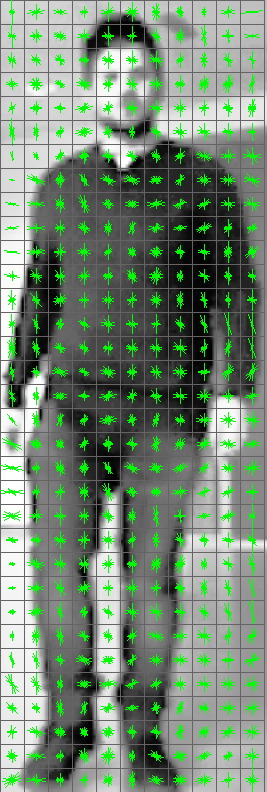
\includegraphics[width=.5\linewidth]{figures/features}
  \caption*{Výpočet příznaků}
  \label{fig:hog_features}
\end{minipage}
\caption{Normalizace a výpočet příznaků pro obrázek}
\label{fig:hogCalc}
\end{figure}

\subsubsection{Support vector machines}

Support vector machines (SVM) jsou učební modely, které jsou velmi populární v oblasti strojového učení. Původně tato technika sloužila k vytvoření optimálního binárního klasifikátoru, později byla rozšířena do regresního a clustering problémů. Tato metoda je založena na tzv. jádrových algoritmech (kernel machines) s využitím podpůrných vektorů (support vectors).

Primárním cílem SVM je nalézt nadrovinu, která optimálně rozděluje prostor příznaků tak, aby trénovací data náležela do konkrétních tříd, viz obrázek \ref{fig:svm}. Pokud mezera mezi oddělující nadrovinou a nejbližšími vektory příznaků z obou kategorií (v případě binárního klasifikátoru) je maximální, jedná se o optimální řešení. Vektory příznaků v blízkosti této nadroviny se nazývají podpůrné vektory, což znamená, že pozice ostatních vektorů nemá vliv na nadrovinu (rozhodovací funkce). 

Jinými slovy, se jedná o diskriminační klasifikátor formálně definovaný rozdělovací nadrovinou, která kategorizuje nové příklady.
\begin{figure}[H]
\centering
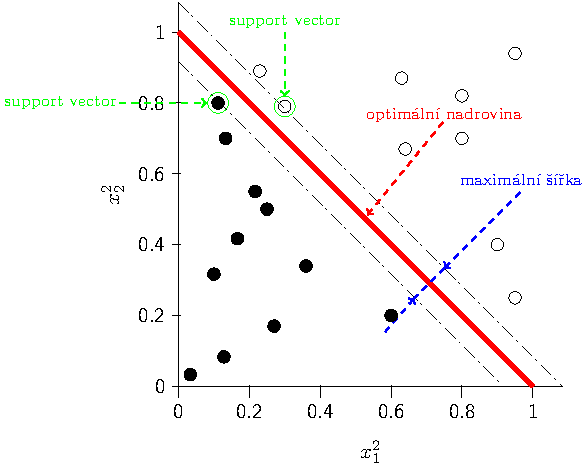
\includegraphics[width=.7\linewidth]{figures/svm.pdf}
\caption{Optimální oddělovací hranice}
\label{fig:svm}
\end{figure}

Implementaci SVM můžeme nalézt již v existujících knihovnách jako jsou například LIBSVM, MATLAB, SAS, SVMLight a další. V následující části bude popsána knihovna LIBSVM, na které je založena implementace v OpenCV a v Dlibu.  

Tato knihovna byla napsána v roce 2001 \cite{libsvm} a stále se vyvíjí. Podporuje různé formulace SVM pro odhady klasifikace, regrese a distribuce.

\paragraph*{$C$-Support vektorová klasifikace (C-SVC)}
Umožnuje nedokonalé oddělení tříd pro n-tříd ($n > 2$) s postihovým multiplikátorem $C$, pro odlehlé hodnoty ($C > 0$). \cite{csvmclass}

\paragraph*{$\nu$-Support vektorová klasifikace ($\nu$-SVC)}
$n$- třídní klasifikace s možností nedokonalé separace. Tato klasifikace přidává nový parametr $\nu \varepsilon (0,1]$ a čím větší je jeho hodnota tím hladší je rozhodovací funkce. \cite{nusvmsvrclass}

\paragraph*{Distribuční odhad (Jednotřídní SVM)}
Distribution Estimation (One-class SVM), jak název, již sám o sobě napovídá, všechny tréninková data pocházejí z jedné třídy, SVM vytvoří hranici, která odděluje třídu od zbývající části. \cite{oneclasssvm}

\paragraph*{$\varepsilon$-Support vektorová regrese ($\varepsilon$-SVR)}
Vzdálenost mezi vektory příznaků a rozdělovací nadrovinou musí být menší než $p (\varepsilon)$. Pro odlehlé hodnoty opět použijeme multiplikátor $C$. Musí tedy platit: $C > 0$ a $\varepsilon > 0$. \cite{svrsvm}

\paragraph*{$\nu$-Support vektorová regrese ($\nu$-SVR)}
Tato klasifikace je podobná jako $\varepsilon$-SVR. Na místo p se použije parametr $\nu \varepsilon (0,1]$. \cite{nusvmsvrclass}

Účinnost SVM závisí na výběru správného jádra a parametry jádra. Nejběžněji se používá Gaussovo jádro s jedním parametrem $\gamma$. V této knihovně se můžeme setkat s následujícími jádry.

\paragraph*{Lineární jádro}
Použití tohoto jádra je velmi rychlé (bez jakékoliv transformace), jedná se lineární diskriminaci a rozdělovací nadrovina bude vždy přímka. Pro toto jádro platí 
\begin{equation*}
 \label{linearK}
  K(x_i, x_j) = x_i^T x_j,
\end{equation*}
  kde $x_i$ a $x_j$ jsou vektory vstupního prostoru.

\paragraph*{Polynomické jádro}
Polynomické jádro umožňuje učení nelineárních modelů
\begin{equation*}
\label{polyK}
  K(x_i, x_j) = (\gamma x_i^T x_j + c)^{d}, \gamma > 0,
\end{equation*}
kde: $c \geq 0$, volný parametr, který vylučuje vliv vyššího řádu oproti polynomu nižšího řádu (pokud $c = 0$, jádro je homogenní), řád polynomu určuje parametr $d$.

\paragraph*{Gaussovo jádro}
Gaussovo neboli RBF (Radial Basis Function) jádro se řadí mezi nejpoužívanější a je definované jako
\begin{equation*}
\label{RBFK}
 K(x_i, x_j) = e^{-\gamma ||x_i - x_j||^2}, \gamma > 0,
\end{equation*}
kde: $||x_i - x_j||^2$ značí kvadratickou euklidovskou vzdálenost mezi dvěma vektory příznaků.

\paragraph*{Sigmoidní jádro}
toto jádro je podobné sigmoidní funkci v logistické regresi
\begin{equation*}
\label{sigmK}
 K(x_i, x_j) = \tanh(\gamma x_i^T x_j + r),
\end{equation*}
kde $r$ je volitelný parametr.

\paragraph*{Exponenciální jádro}
Exponenciální jádro $\chi$2 je podobné RBF jádru a využívá se převážně na histogramy
\begin{equation*}
\label{expK}
 K(x_i, x_j) = e^{-\gamma \chi^2(x_i,x_j)}, \chi^2(x_i,x_j) = \frac{(x_i-x_j)^2}{(x_i+x_j)}, \gamma > 0,
\end{equation*}

\paragraph*{Jádro histogramu průsečíků}
Toto jádro je také známé jako \textit{Min Kernel}, jedná se o nejnovější jádro v této knihovně a je velmi rychlé a užitečné při klasifikaci
\begin{equation*}
\label{innK}
 K(x_i, x_j) = min(x_i,x_j).
\end{equation*}

Nejpoužívanější jádra jsou ilustrována v následujícím obrázku \ref{kernels}.
\begin{figure}[ht] 
  \begin{minipage}[b]{0.5\linewidth}
    \centering
    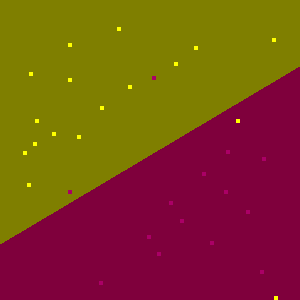
\includegraphics[width=.6\linewidth]{figures/linear} 
    \caption*{Lineární jádro} 
    \vspace{4ex}
    \label{linearKernel} 
  \end{minipage}%%
  \begin{minipage}[b]{0.5\linewidth}
    \centering
    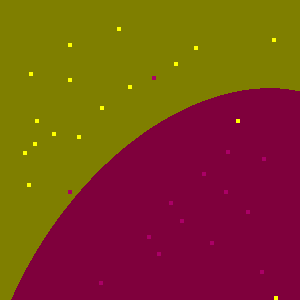
\includegraphics[width=.6\linewidth]{figures/poly} 
    \caption*{Polynomické jádro} 
    \vspace{4ex}
    \label{polyKernel} 
  \end{minipage} 
  \begin{minipage}[b]{0.5\linewidth}
    \centering
    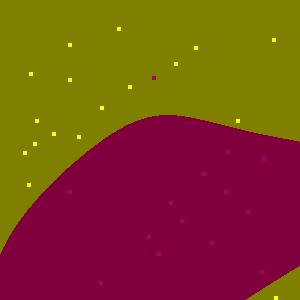
\includegraphics[width=.6\linewidth]{figures/rbf} 
    \caption*{Gaussovo jádro} 
    \vspace{4ex}
    \label{rbfKernel} 
  \end{minipage}%% 
  \begin{minipage}[b]{0.5\linewidth}
    \centering
    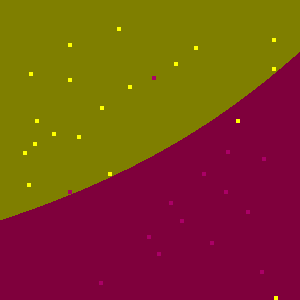
\includegraphics[width=.6\linewidth]{figures/sigm}
    \caption*{Sigmoidní jádro} 
    \vspace{4ex}
    \label{sigmKernel} 
  \end{minipage} 
  \caption{Ilustrační obrázek jader při použití $C$-SVM \cite{libsvm}}
  \label{kernels} 
\end{figure}

SVM je výsledek práce několika lidí po mnoho let. Prvním algoritmem této problematiky je přisuzovaný Vladimíru Vapnikovi v roce 1963 \cite{svm:vapnik}. V reálném životě byly úspěšně použity ve třech hlavních oblastech: kategorizace textu, rozpoznání obrazu a bioinformatika. Mezi konkrétní příklady patří třídění novinových zpráv, rozpoznávání ručně psaných čísel nebo například vzorky rakovinových tkání.

\subsubsection{Kaskádové klasifikátory}
Kaskádový klasifikátor se skládá z více slabších klasifikátorů umístěné v kaskádách za sebou. Požadavky na tento druh klasifikátoru byla rychlost detekce, aby mohl být implementován na procesorech s nižším výkonem, například v kamerách nebo v telefonech. Princip tohoto klasifikátoru je velice jednoduchý a prostý. Klasifikátor na první vrstvě může vyfiltrovat většinu negativních oken. Na druhé vrstvě se mohou odfiltrovat ``těžší'' negativní okna, která přežila z první vrstvy a tak dále. Sub okno, které přežije všechny tyto vrstvy bude označeno jako pozitivní detekce. Příklad řetězce kaskádového klasifikátoru je ilustrován v obrázku \ref{fig:ccpipeline}, kde $K1$-$KN$ je klasifikátor první až n-té vrstvy.

Klasifikátory si mezi sebou předávají všechny informace o vstupním obraze. Tímto kaskádovým vyhodnocováním se může redukovat čas, nutný pro detekci v daném obraze. Prvním takovým klasifikátorem byl detektor obličeje Viola-Jones \cite{violajones}.  
\begin{figure}[H]
\centering
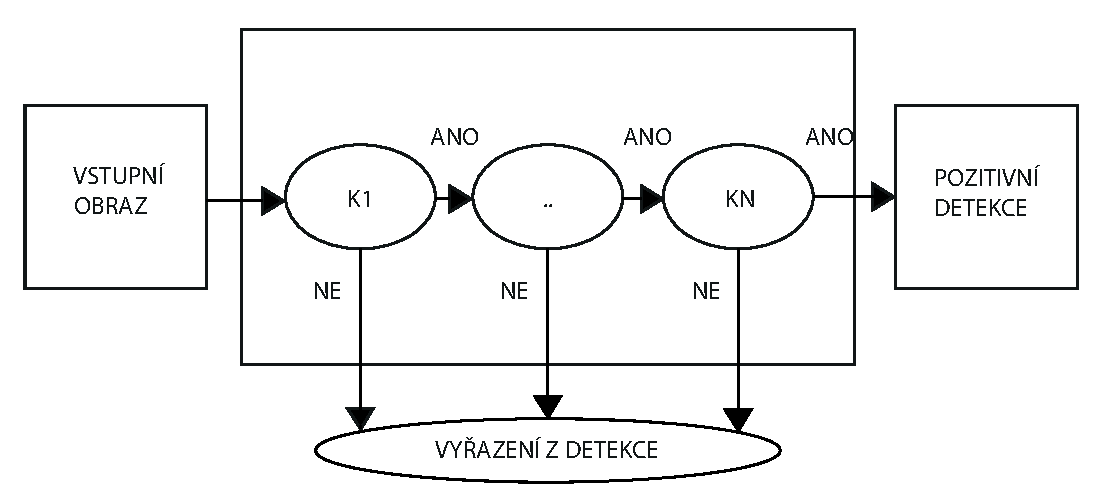
\includegraphics[width=.7\linewidth]{figures/cc.pdf}
\caption{Ukázka pipeline kaskádového klasifikátoru}
\label{fig:ccpipeline}
\end{figure}

\subsubsection{Objektový detektor Viola-Jones}
\textit{Viola-Jones object detector framework} poskytuje v reálném čase spolehlivou a konkurenceschopnou detekci objektů. Tento systém byl navržen v roce 2001 a i když může být vycvičen pro detekci různých objektových tříd, byl primárně použit především pro detekci obličeje. Detektor pracuje s obrazy ve stupně šedi a skládá se ze tří částí. Z integrálního obrazu, Haarových příznaků a AdaBoost algoritmu. 

Integrální obraz je takový obraz (obrázek \ref{fig:integralimage}), kde každý bod $x$ představuje součet hodnot předchozích pixelů doleva a nahoru. Spodní pravý bod obsahuje součet všech pixelů v obraze.
Zápis integrálního obrazu je
\begin{equation*}
\label{integralimage}
 I(x, y) = \sum_{\substack{x' \leq x \\ y' \leq y}}{} i(x', y'),
\end{equation*}
kde $i(x', y')$ je hodnota pixelu na pozici $(x, y)$.
\begin{figure}[H]
\centering
\begin{minipage}{.4\textwidth}
  \centering
  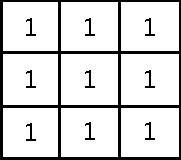
\includegraphics[width=.5\linewidth]{figures/ii_input}
  \caption*{Vstupní obraz}
  \label{fig:ii_input}
\end{minipage}%
\begin{minipage}{.4\textwidth}
  \centering
  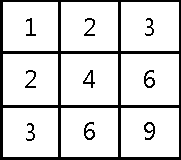
\includegraphics[width=.5\linewidth]{figures/ii_output}
  \caption*{Integrální obraz}
  \label{fig:ii_output}
\end{minipage}
\caption{Převod obrazu na integrální obraz}
\label{fig:integralimage}
\end{figure}


Všechna lidská těla a obličeje sdílejí některé podobné rysy a ty mohou být porovnány pomocí Haarových příznaků.
\begin{itemize}
  \item{Oční oblast je než tmavší než oblast nosního mostu.}
  \item{Proporce lidského těla.}
  \item{Hlava člověka je tmavší než její okolí.}
  \item{Oblast mezi dolními končetinami je světlejší než samotné nohy.}
\end{itemize}
Sada Haarových vlnek je na obrázku \ref{fig:basichaarfeatures}, jedná se pouze o základní sadu příznaků.
\begin{figure}[H]
\centering
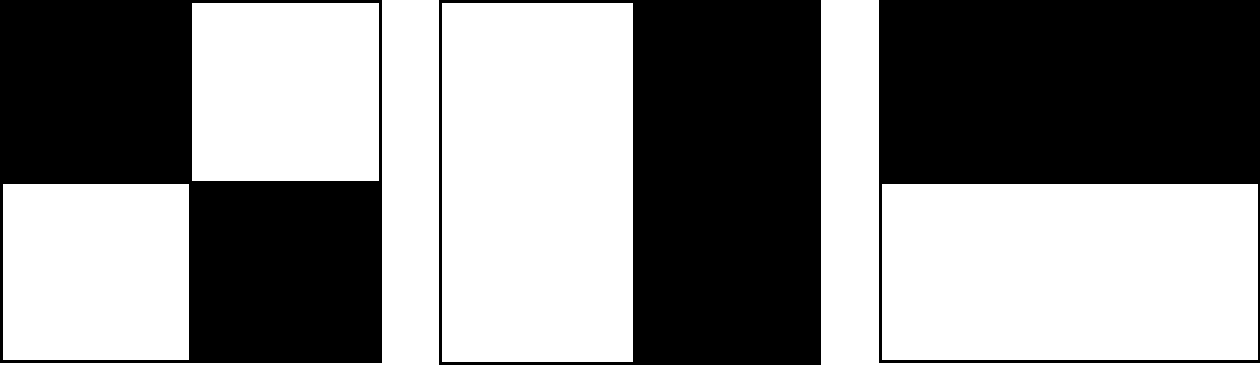
\includegraphics[width=.6\linewidth]{figures/haar_features}
\caption{Základní sada Haarových příznaků}
\label{fig:basichaarfeatures}
\end{figure}

Pro identifikaci lidských postav se používá rozšířená sada vlnek, tzv. Haar-like příznaky. V některých vědeckých publikacích byly představy prototypy těchto příznaků. Na obrázku \ref{fig:haarlike} jsou některé z nich. Hodnota příznaku je rozdíl mezi sumou pixelů pod bílou a černou oblastí Haarových vlnek.
\begin{figure}[H]
\centering
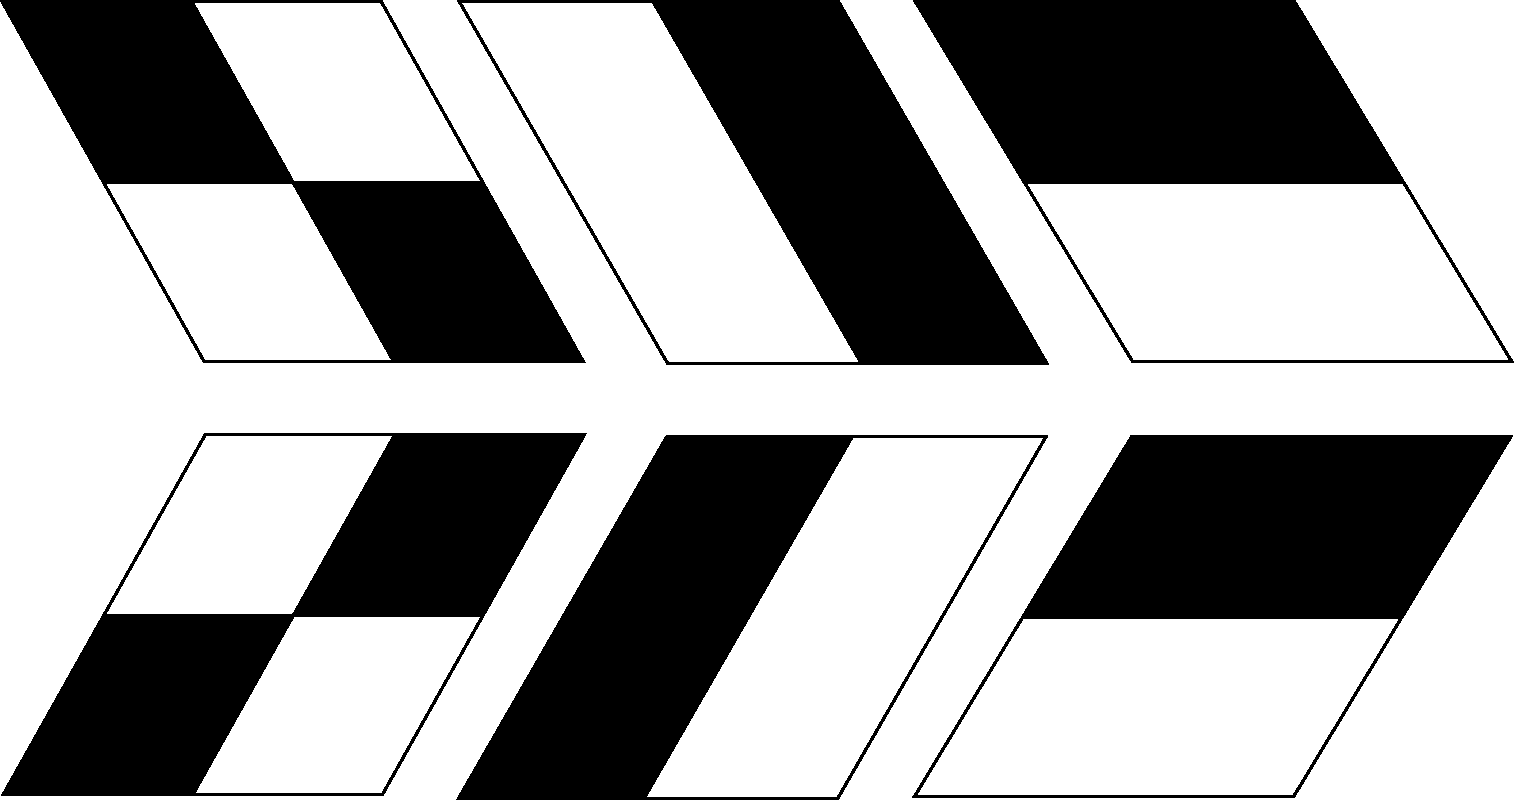
\includegraphics[width=.5\linewidth]{figures/haar_like}
\caption{Vybrané prototypy Haar-like příznaků}
\label{fig:haarlike}
\end{figure}

\textbf{AdaBoost}, neboli Adaptive Boosting byl představen v práci pánů Freund a Schapire \cite{adaboost}. Tento klasifikátor kombinuje slabé klasifikátory k vytvoření jednoho silného klasifikátoru. V kombinaci více klasifikátorů s výběrem trénovací sady v každé iteraci algoritmu a přidělení správné váhy na konci trénování, docílíme klasifikátoru s dobrou přesností. Klasifikátory v tomto řetězci, které mají klasifikační přesnost menší než 50\% jsou ohodnoceny zápornou vahou. Váhou nula jsou ohodnoceny klasifikátory, které mají přesnost 50\%. Pouze ty, co mají přesnost vyšší než 50\% jsou přínosné do této kombinace a můžeme hovořit o zesílení (boosting) klasifikace. 

\subsubsection{Lokální binární vzor}
Metoda LBP (Local Binary Pattern) byla navržena pro klasifikaci textur v obrazech v roce 1990. \cite{lbp:texture} Poprvé však byly popsány až v roce 1994. \cite{lbp:first} Hlavní myšlenkou LBP, že struktury obrazu mohou být efektivně zakódovány porovnání všech pixelů se sousedními pixely. Výsledkem

Prvním krokem této metody je převod obrazu do stupně šedi a jeho rozdělení do buněk. Okolní hodnoty pixelů jsou porovnávány se středovým pixelem, pokud je jejich hodnota rovna nebo větší zapíše se na tuto pozici jednička v opačném případě nula. Tyto hodnoty seřadíme buď podle hodinových ručiček nebo naopak a získáme 8-místné binární číslo, které převedeme do dekadické soustavy. Následujícím kroku z čísel, které jsme získali kombinací pixelů v buňkách vypočítáme histogram. V posledním kroku zřetězíme všechny histogramy buněk a získáme vektor příznaků pro celý obraz. Jedná se o 256-dimenzionální vektor příznaků. 
Matematicky lze LPB vyjádřit jako
\begin{equation*}
LBP_{P,R} = \sum_{p=0}{P-1} s(g_p - g_c)2^P, \\
s(x) =
  \begin{cases} 
   1 & \text{pro } x \geq 0 \\
   0       & \text{pro } x < 0
  \end{cases}
\end{equation*}
kde: $P$ je počet bodů v okolí, $R$ vyjadřuje vzdálenost bodů od středového pixelu, $g_c$ je středový pixel $g_p$ je aktuální pixel. 

Následující příklad se vztahuje k obrázku \ref{fig:lbpsum}. Po porovnání pixelů se středovým pixelem, jsme získali vzor $11110001$. Tento vzor převedeme do dekadické soustavy a sečteme, $ 1+16+32+64+128 = \textbf{241}$. Získali jsme hodnotu této buňky do vektoru příznaků.

\begin{figure}[H]
\centering
\begin{minipage}[b]{.3\textwidth}
  \centering
  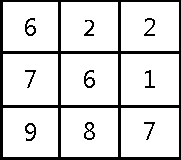
\includegraphics[width=.5\linewidth]{figures/lbp_img}
  \caption*{Vstupní buňka}
  \label{fig:lpbimg}
\end{minipage}%
\begin{minipage}[b]{.3\textwidth}
  \centering
  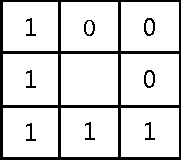
\includegraphics[width=.5\linewidth]{figures/lbp_thresh}
  \caption*{Prahové hodnoty}
  \label{fig:lbpthresh}
\end{minipage}
\begin{minipage}[b]{.3\textwidth}
  \centering
  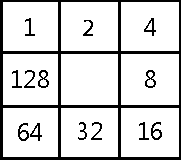
\includegraphics[width=.5\linewidth]{figures/lbp_weights}
  \caption*{Váhově ohodnoceny pixely}
  \label{fig:lbpweights}
\end{minipage}
\caption{Výpočet příznaku}
\label{fig:lbpsum}
\end{figure}

Výhoda této metody je její rychlý a snadný výpočet a odolnost vůči různým osvětlením. Na druhou stranu je těžší na trénování, protože výsledné dekadické číslo může mít obrovské množství možností (podle parametru $P$). K omezení můžeme využít uniformní vzory (viz obrázek \ref{fig:lbpvzory}), které vyfiltrují možné okolí. Pro parametr $P=8$, získáme 59 vzorů. 

\begin{figure}[H]
\centering
\begin{minipage}[b]{.17\textwidth}
  \centering
  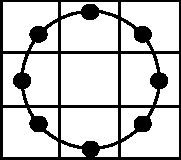
\includegraphics[width=.9\linewidth]{figures/lbp_spot}
  \caption*{Spot}
\end{minipage}
\begin{minipage}[b]{.17\textwidth}
  \centering
  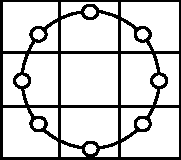
\includegraphics[width=.9\linewidth]{figures/lbp_spot_flat}
  \caption*{Spot/Flat}
\end{minipage}
\begin{minipage}[b]{.17\textwidth}
  \centering
  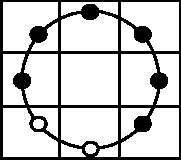
\includegraphics[width=.9\linewidth]{figures/lbp_line}
  \caption*{Line}
\end{minipage}
\begin{minipage}[b]{.17\textwidth}
  \centering
  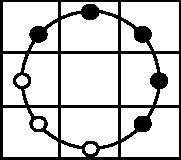
\includegraphics[width=.9\linewidth]{figures/lbp_corner}
  \caption*{Corner}
\end{minipage}
\begin{minipage}[b]{.17\textwidth}
  \centering
  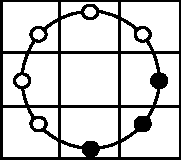
\includegraphics[width=.9\linewidth]{figures/lbp_edge}
  \caption*{Edge}
\end{minipage}
\caption{Lokální okolí LBP metody}
\label{fig:lbpvzory}
\end{figure}

Pro detekování chodců v obrazech se LPB kombinují s metodou HOG. \cite{hoglpb}